\documentclass[12pt]{report}
\usepackage{../mystyle}
\begin{document}
\boldmath
\pagestyle{fancy}

\chapter{Linear Algebra for Data Science. \\[-1cm] \hspace*{3.5cm} \large Work has been done by: Ryabykin Aleksey. Variant 42\vskip3.2ex}
\fancyhead[L]{Graded Homework 1.}
\fancyhead[C]{Linear Algebra for Data Science}
\fancyhead[R]{Ryabykin Aleksey (Variant 42)}
% \setcounter{subsection}{2}
\begin{problem}{}
 Find the SVD decomposition and, using it, the pseudoinverse of the matrix:
 \[
   \begin{bmatrix}
    -46 & -3 & 68 & -28\\
    2 & 54 & -76 & 32 \\
    25 & -102 & -20 & -44 
 \end{bmatrix}.
 \]   
\end{problem}

\begin{solution}
    Let's start with finding the matrix $V \in M_{4\times 4}(\R)$ and $\Sigma \in M_{3\times 4}(\R)$:
    \[
         A^\intercal A = \begin{bmatrix}
            -46 & 2 & 25 \\
            -3 & 54 & -102 \\
            68 & -76 & -20 \\
            -28 & 32 & -44
         \end{bmatrix}  \begin{bmatrix}
            -46 & -3 & 68 & -28\\
            2 & 54 & -76 & 32 \\
            25 & -102 & -20 & -44 
         \end{bmatrix} = \begin{bmatrix}
            2745  & -2304  & -3780  &  252 \\
           -2304  &  13329  & -2268  &  6300 \\
           -3780  & -2268  &  10800  & -3456 \\
            252  &  6300  & -3456  &  3744 
          \end{bmatrix}
    \]
    Lets find the eigenvalues needed to find the singular values and eigenvectors:
    \[
          |A^TA - \lambda I| = 0
    \]
    Solving this equation, we can obtain eigenvalues:
    \[
      \begin{array}{cc}
         \lambda_1 = 18225, & \ \lambda_2 = 11664 \\       
         \lambda_3 = 729 & \lambda_4 = 0  
      \end{array}
    \]
    Let me take a square root of the nonzero eigenvalues:
    \[
      \begin{array}{cc}
         \lambda_1 = 135, & \ \lambda_2 = 108 \\       
         \lambda_3 = 27  
      \end{array}
    \]
    Then the $\Sigma$ matrix is a zero matrix with $\sigma_i$ on its diagonal:  
    \[
         \Sigma = \begin{bmatrix}
            135 & 0 & 0 & 0\\
            0 & 108 & 0 & 0\\
            0 & 0 & 27 & 0
         \end{bmatrix}
    \]
    Now lets find the eigenvectors for each eigenvalue:
    \begin{itemize}
      \item $\lambda = 18225$:
      \[
         \vec{v}_1 = \begin{bmatrix}
            0 & \dfrac{7}{4} & -1 & 1
         \end{bmatrix}^\intercal
      \]
      To normalize it we need to multiply it by its norm: $||\vec{v}_1|| = \dfrac{9}{4}$.
      \item $\lambda = 11664$:
      \[
         \vec{v}_2 = \begin{bmatrix}
            -\dfrac{4}{7} & \dfrac{4}{7} & 1 & 0
         \end{bmatrix}^\intercal
      \]
      $||\vec{v}_2|| = \dfrac{9}{7}$.
      \item $\lambda = 729$:
      \[
         \vec{v}_3 = \begin{bmatrix}
            -\dfrac{7}{4} & 0 & 1 & 1
         \end{bmatrix}^\intercal 
      \]
      $||\vec{v}_3|| = \dfrac{9}{4}$
      \item $\lambda = 0$:
      \[
         \vec{v}_4 = \begin{bmatrix}
            -\dfrac{4}{7} & -\dfrac{4}{7} & 0 & 1
         \end{bmatrix}^\intercal.
      \]
      $||\vec{v}_4|| = \dfrac{9}{7}$
    \end{itemize}
    Normalized vectors $v_i, \ i \in \{1, \ldots, 4\}$ make up the matrix $V$:
    \[
         V = \begin{bmatrix}
            0 & -\medmath{\dfrac{4}{9}} & \medmath{\dfrac{7}{9}} & -\medmath{\dfrac{4}{9}} \\[0.2cm]
            \medmath{\dfrac{7}{9}} & \medmath{\dfrac{4}{9}} & 0 & -\medmath{\dfrac{4}{9}} \\[0.2cm]
            -\medmath{\dfrac{4}{9}} & \medmath{\dfrac{7}{9}} & \medmath{\dfrac{4}{9}} & 0 \\[0.2cm]
            \medmath{\dfrac{4}{9}} & 0 & \medmath{\dfrac{4}{9}} & \medmath{\dfrac{7}{9}}
         \end{bmatrix}
    \]
    Now we can express vectors $u_i$ from matrix $U$ in terms of $v_i$:
    \[
         u_i = \dfrac{1}{\sigma_i} \cdot v_i
    \]
    So:
    \[
         \begin{array}{c}
            u_1 = \dfrac{1}{135} \begin{bmatrix}
               -46 & -3 & 68 & -28\\
               2 & 54 & -76 & 32 \\
               25 & -102 & -20 & -44 
            \end{bmatrix} \cdot \begin{bmatrix}
               0 & \dfrac{7}{9} & -\dfrac{4}{9} & \dfrac{4}{9}^\intercal 
            \end{bmatrix} = \begin{bmatrix}
                  -\dfrac{1}{3} & \dfrac{2}{3} & -\dfrac{2}{3}
               \end{bmatrix}^\intercal \\[1.5cm]
               u_2 = \dfrac{1}{108} \begin{bmatrix}
                  -46 & -3 & 68 & -28\\
                  2 & 54 & -76 & 32 \\
                  25 & -102 & -20 & -44 
               \end{bmatrix} \begin{bmatrix}
                  -\dfrac{4}{9} & \dfrac{4}{9} & \dfrac{7}{9} & 0
               \end{bmatrix}^\intercal = \begin{bmatrix}
                  \dfrac{2}{3} & -\dfrac{1}{3} & -\dfrac{2}{3}
               \end{bmatrix}^\intercal \\[1.5cm]
               u_3 = \dfrac{1}{27} \begin{bmatrix}
                  -46 & -3 & 68 & -28\\
                  2 & 54 & -76 & 32 \\
                  25 & -102 & -20 & -44 
               \end{bmatrix} \begin{bmatrix}
                  \dfrac{7}{9} & 0 & \dfrac{4}{9} & \dfrac{4}{9}
               \end{bmatrix}^\intercal = \begin{bmatrix}
                  -\dfrac{2}{3} & -\dfrac{2}{3} & -\dfrac{1}{3}
               \end{bmatrix}^\intercal
         \end{array}
    \]
    Therefore, 
    \[
         U = \begin{bmatrix}
            -\dfrac{1}{3} & \dfrac{2}{3} & -\dfrac{2}{3}\\[0.25cm] 
            \dfrac{2}{3} & -\dfrac{1}{3} & -\dfrac{2}{3}\\[0.25cm]
            -\dfrac{2}{3} & -\dfrac{2}{3} & -\dfrac{1}{3}
         \end{bmatrix}
    \]
    Finally, 
    \[
       A^+ = V\Sigma^+U^* = \begin{bmatrix}
         -0.021948 & -0.017833 & -0.006859\\
          0.000823 &  0.002469 & -0.006584\\
         -0.005075 & -0.015569 & -0.008093\\
         -0.012071 & -0.008779 & -0.007682
        \end{bmatrix}
    \]
\end{solution}

\begin{problem}{}
  Find a full rank decomposition and the pseudoinverse of the matrix:
  \[
      A = \begin{bmatrix}
         -1 & 5 & 8\\
         4 & -15 & -12\\
         3 & -11 & -8\\
         -2 & 9 & 12
      \end{bmatrix}.
  \]
\end{problem}

\begin{solution}
   Let's start with finding a full rank decomposition of a matrix $A$ and then we will obtain the pseudoinverse matrix by the formula:
   \[
        A^+ = G^*(G,G^*)^{-1}(F^*,F)^{-1}F^* 
   \]
   So let me go through finding the reduced row echelon form of a matrix $A$:
   \[
      \begin{array}{c}
         \displaystyle A = \Vast[
            \overbrace{\fbox{$\begin{matrix}
                -1 & 5 \\
                4 & -15 \\
                3 & -11 \\
                -2 & 9
            \end{matrix}$}}^{F} \hspace*{0.25cm} \begin{matrix}
                8 \\
                -12 \\
                -8 \\
                12
            \end{matrix}\Vast] \Rightarrow \begin{bmatrix}
            1 & -5 & -8\\
            4 & -15 & -12\\
            3 & -11 & -8\\
            -2 & 9 & 12
         \end{bmatrix} \Rightarrow \begin{bmatrix}
            1 & -5 & -8\\
            0 & 5 & 20\\
            0 & 4 & 16\\
            0 & -1 & -4
         \end{bmatrix} \Longrightarrow \\[1.25cm]
         \displaystyle \Rightarrow \begin{bmatrix}
            1 & -5 & -8\\
            0 & 1 & 4\\
            0 & 0 & 0\\
            0 & 0 & 0
         \end{bmatrix} \Rightarrow \VVast[\begin{tabular}{c} \\[-1cm]
            $\overbrace{\fbox{\begin{tabular}{ccc}
               $1$ & $0$ & $12$\\
               $0$ & $1$ & $4$ \\[-0.1cm]
            \end{tabular}}}^G$ \\
            \hspace*{-0.3cm} \begin{tabular}{ccc}
               $0$ & $0$ & $0$\\
               $0$ & $0$ & $0$
            \end{tabular}
            \end{tabular}\Vast]
      \end{array}
   \]
   We have obtained the full rank decomposition, lets check whether is it correct:
   \[
      A  = F \cdot G = \begin{bmatrix}
         -1 & 5 \\
         4 & -15 \\
         3 & -11 \\
         -2 & 9
      \end{bmatrix} \cdot \begin{bmatrix}
         1 & 0 & 12\\
         0 & 1 & 4
      \end{bmatrix} = \begin{bmatrix}
         -1 & 5 & 8\\
         4 & -15 & -12\\
         3 & -11 & -8\\
         -2 & 9 & 12
      \end{bmatrix}
   \]
   This identity is correct. Keeping in mind, that our matrices are defined on the real numbers field, the Hermitian transposed matrix means just transposed. Now we can obtain the pseudoinverse matrix to $A$. Let me do it step by step:
   \[
      G^*\left(G, G^*\right)^{-1} = \begin{bmatrix}
         1 & 0 \\
         0 & 1\\
         12 & 4 
      \end{bmatrix} \cdot \left(\begin{bmatrix}
         1 & 0 & 12\\
         0 & 1 & 4
      \end{bmatrix} \cdot \begin{bmatrix}
         1 & 0 \\
         0 & 1\\
         12 & 4 
      \end{bmatrix}\right)^{-1} = \begin{bmatrix}
         1 & 0 \\
         0 & 1\\
         12 & 4 
      \end{bmatrix} \cdot \dfrac{1}{161}\begin{bmatrix}
         17 & -48 \\
         -48 & 145
      \end{bmatrix} = \dfrac{1}{161} \begin{bmatrix}
         17 & -48 \\
         -48 & 145 \\
         12 & 4
      \end{bmatrix}.
   \]
   And next step:
   \[
      \dfrac{1}{161} \begin{bmatrix}
         17 & -48 \\
         -48 & 145 \\
         12 & 4
      \end{bmatrix} \left(F^*, F\right)^{-1} = \dfrac{1}{161} \begin{bmatrix}
         17 & -48 \\
         -48 & 145 \\
         12 & 4
      \end{bmatrix} \dfrac{1}{104} \begin{bmatrix}
         452 & 116 \\
         116 & 30
      \end{bmatrix} = \dfrac{1}{16744} \begin{bmatrix}
         2116 & 532\\
         -4876 & -1218\\
         5888 & 1512
      \end{bmatrix}
   \]
   And the last step:
   \[
      \dfrac{1}{16744} \begin{bmatrix}
         2116 & 532\\
         -4876 & -1218\\
         5888 & 1512
      \end{bmatrix} \cdot \begin{bmatrix}
         -1 & 4 & 3 & -2\\
         5 & -15 & -11 & 9
      \end{bmatrix} = \dfrac{1}{16744} \begin{bmatrix}
         544 & 484 & 496 & 556 \\
         -1214 & -1234 & -1230 & -1210 \\
         1672 & 872 & 1032 & 1832
      \end{bmatrix} = A^+
   \]
   % Lets check the correctness of the computing by the Penrose axioms:
   % \begin{enumerate}
   %    \item $AA^+A = A$:
   %    \[
   %       \begin{array}{c}
   %       \displaystyle \dfrac{1}{16744}\begin{bmatrix}
   %          -1 & 5 & 8\\
   %          4 & -15 & -12\\
   %          3 & -11 & -8\\
   %          -2 & 9 & 12
   %       \end{bmatrix} \begin{bmatrix}
   %             544 & 484 & 496 & 556 \\
   %             -1214 & -1234 & -1230 & -1210 \\
   %             1672 & 872 & 1032 & 1832
   %       \end{bmatrix}
   %       \begin{bmatrix}
   %          -1 & 5 & 8\\
   %          4 & -15 & -12\\
   %          3 & -11 & -8\\
   %          -2 & 9 & 12
   %       \end{bmatrix} \\
   %       \displaystyle \dfrac{1}{16744}\begin{bmatrix}
   %          -16744 & 83720 & 1333952\\
   %          66976 & -251160 & -200928\\
   %          50232 & -184184 & -133952 \\
   %          -33488 & 150696 & 200928
   %       \end{bmatrix} = \begin{bmatrix}
   %          -1 & 5 & 8\\
   %          4 & -15 & -12\\
   %          3 & -11 & -8\\
   %          -2 & 9 & 12
   %       \end{bmatrix}
   %    \end{array}
   %    \]
   % \end{enumerate}
\end{solution}

\begin{problem}{}
   Find the general formula for the solutions of the following system using the least squares method and among them find the smallest length:
   \[
      \left\{
         \begin{array}{c}
            -2\cdot x + 10\cdot y + 13\cdot z - 5\cdot t = 1\\
            4 \cdot x - 14\cdot y - z + 11\cdot t = 6\\
            3\cdot x - 10\cdot y + 0\cdot z + 15\cdot t = 9\\
            -1\cdot x + 6 \cdot y + 12 \cdot z - 9\cdot t = 4 
         \end{array}
      \right.
   \]
\end{problem}

\begin{solution}
   Our goal in this case is to find all pseudosolutions using the following formula:
   \[
      \vec{v} = A^+\vec{b} - (A^+A - I) \vec{a}, 
   \]
   where $A \in M_{4 \times 4}$ is a matrix of the coefficients of the given system, $\vec{b} \in \R^4$ -- known right side vector, $\vec{a}$ is an arbitrary vector. And keeping in mind, that the pseudosolution $\hat{u} = A^+ \vec{b}$ has the minimal length, we can solve the remaining task. Firstly, we need to find a pseudoinverse matrix. Let me do it by a full rank decomposition. Let's write the matrix of the coefficients of the system:
   \[
       A = \begin{bmatrix}
         -2 & 10 & 13 & -5 \\
         4 & -14 & -1 & 11 \\
         3 & -10 & 0 & 15 \\
         -1 & 6 & 12 & -9
       \end{bmatrix}, \hspace*{0.5cm} \vec{b} = \begin{bmatrix}
         1 & 6 & 9 & 4
       \end{bmatrix}^\intercal
   \] 
   First step is to get the reduced echelon form of the matrix:
   \[
       A = 
       \Vast[
            \overbrace{\fbox{$\begin{matrix}
                -2 & 10 & 13 \\
                4 & -14 & -1 \\
                3 & -10 & 0 \\
                -1 & 6 & 12
            \end{matrix}$}}^{F} \hspace*{0.25cm} \begin{matrix}
                -5 \\
                11 \\
                15 \\
                -9
            \end{matrix}\Vast] 
        \Rightarrow \begin{bmatrix}
         1 & 0 & 0 & 75 \\
         0 & 1 & 0 & 21 \\
         0 & 0 & 1 & -5 \\
         0 & 0 & 0 & 0
       \end{bmatrix}
       \VVast[\begin{tabular}{c} \\[-1cm]
         $\overbrace{\fbox{\begin{tabular}{cccc}
            $1$ & $0$ & $0$ & $75$\\
            $0$ & $1$ & $0$ & $21$ \\
            $0$ & $0$ & $1$ & $-5$\\ [-0.1cm]
         \end{tabular}}}^G$ \\
         \hspace*{-0.3cm} \begin{tabular}{cccc}
            $0$ & $0$ & $0$ & $0$
         \end{tabular}
         \end{tabular}\Vast]
   \]
   \[
   A^+ = G^*\left(G, G^*\right)^{-1}(F^*, F)^{-1}F^* = \dfrac{1}{97472} \begin{bmatrix}
      -1244 & 2416 & -877 & 2049 \\
      5500 & -8096 & 3897 & -6493 \\
      3332 & 3088 & 1683 & 4737 \\
      5540 & -4256 & 7647 & -6363
   \end{bmatrix}.
   \]
   Now we can find the smallest pseudosolution:
   \[
      \hat{u} = A^+ \vec{b} = \begin{bmatrix}
         0.14 & -0.35 & 0.574 & 0.24
      \end{bmatrix}^\intercal
   \]
   All pseudosolutions:
   \[
      \begin{array}{c}
         \displaystyle 
         \vec{v} =  \begin{bmatrix}
            0.14 \\ -0.35 \\ 0.574 \\ 0.24
         \end{bmatrix} - \begin{bmatrix}
            -0.92 & -0.259 & 0.062 & 0.012 \\
            -0.259 & -0.0724 & 0.017 & 0.00345 \\
            0.062 & 0.017 & -0.004 & -0.0008 \\
            0.012 & 0.00345 & -0.0008 & -0.0002
         \end{bmatrix}\cdot \begin{bmatrix}
            a_1 \\ a_2 \\ a_3 \\ a_4
         \end{bmatrix} \\[1cm]
         \displaystyle
         = \begin{bmatrix}
            0.14 + 0.92 a_1 + 0.259 a_2 -0.062 a_3 - 0.012 a_4\\
            -0.35 + 0.259a_1 + 0.0724a_2 - 0.017a_3 + 0.00345 a_4 \\
            0.574 - 0.062 a_1 - 0.017 a_2 + 0.004 a_3 + 0.0008 a_4 \\
            0.24 - 0.012 a_1 - 0.00345 a_2 + 0.0008 a_3 + 0.0002 a_4
         \end{bmatrix}.
      \end{array}
   \]
\end{solution}

\begin{problem}{}
    Find an interpolation polynomial that pases through the four points whose coordinates form the columns of the matrix:
    \[
         P = \begin{bmatrix}
            -2 & -1 & 0 & 2\\
            17 & 5 & -14 & -11
         \end{bmatrix}.
    \]
\end{problem}

\begin{solution}
    Lagrange form of interpolation polynomial:
    \[
    f(x) = \sum\limits_{i=0}^{3}y_i \dfrac{(x-x_0)\ldots(x-x_{i-1})(x-x_{i+1})\ldots (x-x_n)}{(x_i - x_0)\ldots (x_i - x_{i-1})(x_i - x_{i+1})\ldots (x_i - x_n)},  
\]
where $\vec{x} = \begin{bmatrix}
   x_i
\end{bmatrix}, \ i = \{0, \ldots, 3\}$ is the first row of the given matrix, $\vec{y} = \begin{bmatrix}
   y_i
\end{bmatrix}, \ i = \{0, \ldots, 3\}$ is the second row of the given matrix. We can finally obtain it:
\[
   \begin{array}{c}
      \displaystyle 17 \cdot \dfrac{(x+1) x (x-2)}{(-2 + 1) (-2 - 0) (-2 - 2)} + 5 \cdot \dfrac{(x+2) x (x-2)}{(-1 + 2) (-1) (-1 - 2)} - \\[0.5cm]
      \displaystyle - 14\cdot \dfrac{(x+2) (x+1) (x-2)}{(0 + 2)(0 + 1) (0 - 2)} - 11 \cdot \dfrac{(x+2) (x+1) x}{(2 + 2) (2 + 1) 2}       
   \end{array}
\]
Making some simplifications:
\[
   \begin{array}{c}
      \displaystyle -\dfrac{17}{8}\left(x^3 - x^2 - 2x\right) + \dfrac{5}{3} \left(x^3 - 4x\right) + \dfrac{14}{4} \left(x^3 - 4x + x^2 -4\right) - \dfrac{11}{24} \left(x^3 + 3x^2 + 2x\right) = \\ 
      \displaystyle = \dfrac{1}{24}\left(-51x^3 + 51x^2 + 102x + 40x^3 - 160x + 84x^3 -336x + 84x^2 -336 - 11x^3 - 33x^2 - 22x\right) = \\
      \displaystyle = \dfrac{1}{24}\left(62x^3 + 102x^2 - 416x - 336\right)
   \end{array}
\]
So, we can finnaly obtain the interpolation polynomial:
\[
   f(x) = \dfrac{31}{12}x^3 + \dfrac{51}{12}x^2 - \dfrac{52}{3}x - 14.
\]
\end{solution}

\begin{problem}{}
    Find a (parametric) equation defining the Bézier curve defied by the four points whose coordinates form the columns of the matrix. Sketch the curve on the coordinate plane:
    \[
         P = \begin{bmatrix}
            3 & 6 & 8 & 9\\
            5 & 9 & 6 & 9
         \end{bmatrix}.
    \]
\end{problem}

\begin{solution}
      Explicit formula for Bézier curve:
      \[
          B(t) = \sum\limits_{i=0}^3 P_i \cdot b_{n,i}(t),  
      \]
      where $P_i$ -- points with coordinates in the given matrix $P$, $b_{n,i}$ -- Bernstein polynomials of a kind:
      \[
          b_{n,i} = C_n^i (1-t)^{n-i}t^i   
      \]
      So, we have:
      \[
         \begin{array}{c}            
         \displaystyle B(t) = \begin{bmatrix}
            3 \\ 5
         \end{bmatrix} C_3^0 (1-t)^3t^0 + \begin{bmatrix}
            6 \\ 9
         \end{bmatrix} C_3^1 (1-t)^2t^1 + \begin{bmatrix}
            8 \\ 6
         \end{bmatrix} C_3^2 (1-t)^1t^2 + \begin{bmatrix}
            9 \\ 9
         \end{bmatrix} C_3^3 (1-t)^0 t^3 = \\[0.5cm]
         \displaystyle = \begin{bmatrix}
            3 - 9t + 9t^2 -3t^3 + 18t^3 - 36t^2 + 18t + 24t^2 - 24t^3 + 9t^3 \\
            5 - 15t + 15t^2 - 15t^3 + 27t^3 - 54t^2 + 27t + 18t^2 - 18t^3 + 9t^3
         \end{bmatrix} = 
      \end{array}
      \]
      And after simplifications:
      \[
         B(t) = \begin{bmatrix}
            - 3t^2 + 9t + 3\\
            13t^3 - 21t^2 + 12t + 5
         \end{bmatrix}
      \]
      \begin{figure}[H]
         \centering
         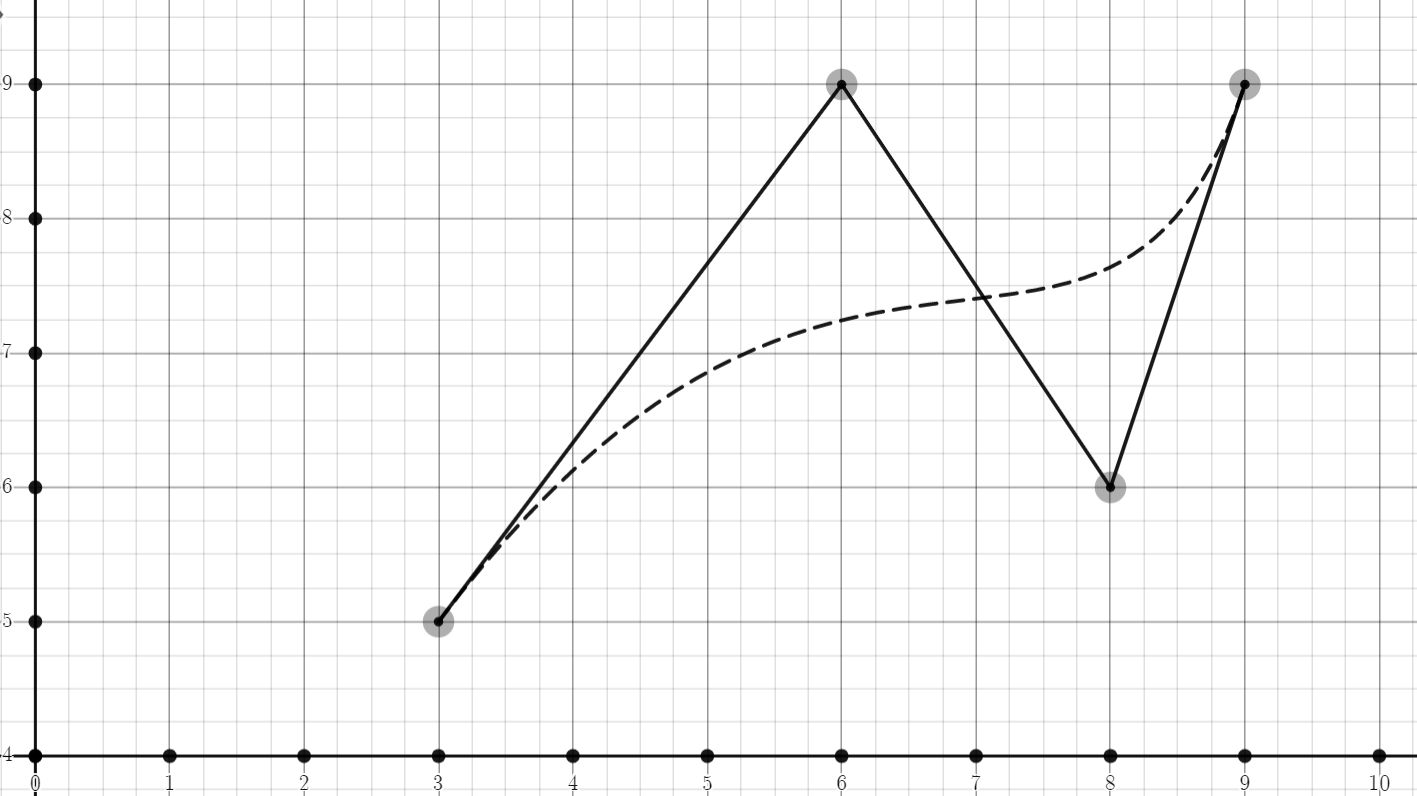
\includegraphics[scale=0.6]{images/bezier.png}
         \caption*{Bézier curve on the coordinate plane}
      \end{figure}
\end{solution}

\begin{problem}{}
    For the polynomial $x^3 + 3x^2 - 4x - 6$ find the best approximation with respect to the max-norm: $\displaystyle \int\limits_1^3 |f(x)|dx$ by a polynomial of degree $2$ on a line segment $[1;3]$.
\end{problem}

\begin{solution}
    In case of such norm we need to use the knowledge of Chebyshev polynomials of second kind. So, we do have some preliminary information:
    \[
         \tilde{U}_n (x) = \dfrac{1}{2^n} U_n(x) 
    \]
    is the area under the curve on segment $[-1, 1]$. For our segment we do need to change the variables:
    \[
         \tilde{U}_n (x) = \dfrac{(b-a)^n}{2^{2n}} U_n \left(\dfrac{2x - (b+a)}{b-a}\right).
    \]
    We are looking for the best approximation by a polynomial of degree $2$, then $n = 3$, $a = 1, \ b = 3$:
    \[
         \tilde{U}_3(x) = \dfrac{2^3}{2^6} U_3 \left(\dfrac{2x - 4}{2}\right).
    \]
    Keeping in mind, that $U_3(x) = 8x^3 - 4x$, we can obtain:
    \[
         \dfrac{1}{8} \cdot 8 \left(\dfrac{2x-4}{2}\right)^3 - \dfrac{1}{8} \cdot 4 \cdot \dfrac{2x-4}{2} = (x-2)^3 - \dfrac{1}{2} x - 1 = x^3 - 6x^2 + 12x - 8 - \dfrac{x}{2} - 1 = x^3 - 6x^2 + \dfrac{23}{2} x - 9.
    \]
    Let me denote the given polynomial as $G$. Then:
    \[
         \tilde{U}_3(x) = G(x) - P_2(x)
    \]
    Let's calculate $P_2(x)$:
    \[
      \begin{array}{c}
         \displaystyle P_2(x) = G(x) - \tilde{U}_3(x) = x^3 + 3x^2 - 4x - 6 - x^3 + 6x^2 - \dfrac{23}{2}x + 9 = 
         \\
         \displaystyle = 9x^2 - \dfrac{31}{2}x + 3
      \end{array}
    \]
\end{solution}

\begin{problem}{}
    Find a polynomial of degree $\leq 3$ that approximates the function $f(x) = \sqrt{2x+5}$ on the segment $[1;6]$ in the norm: $\displaystyle |h|_T = \sqrt{\int\limits_{1}^6 \dfrac{h(x)^2}{\sqrt{1 - (2x-7)^2/25}}dx}
    $
\end{problem}

\begin{solution}
    Because we have the segment $[1;6]$, then, similarly to the previous problem, we need to change variables:
    \[
         y = \dfrac{a+b}{2} + \dfrac{b-a}{2}x = \dfrac{7}{2} + \dfrac{5}{2}x
    \]
    Now we can substitute the new variable into the given norm:
    \[
         |h|_T = \sqrt{\displaystyle \int\limits_{-1}^1\dfrac{h\left(\dfrac{7}{2} + \dfrac{5}{2}x\right)^2}{\sqrt{1-x^2}}dx}
    \]
    The best approximation of a function $f$ by polynomial of degree $\leq n$:
    \[
         \tilde{f}(x) = \sum\limits_{i=0}^3 \dfrac{\langle T_i, f \rangle}{\langle T_i, T_i \rangle} T_i(x).
    \]
    With a corresponding scalar product:
    \[
         \langle f, g \rangle = \int\limits_{-1}^1 \dfrac{f(x)g(x)}{\sqrt{1-x^2}}dx
    \]
    But as we made a change of variable we must must take this into account and return it back to the first one. That is why:
    \[
         f(x) = \sum\limits_{i=0}^3 \dfrac{\big\langle T_i(x), f\left(\dfrac{7}{2} + \dfrac{5}{2}x
         \right) \big\rangle}{\langle T_i(x), T_(x) \rangle} T_i\left(\dfrac{2x - 7}{5}\right)
    \]
    Let me do it iteratively, step by step. For every step we need: $f\left(\dfrac{7}{2} + \dfrac{5}{2}x\right) = \sqrt{5x+12}$ and knowledge about orthogonality relations:
    \[
         \langle T_m, T_n \rangle = \left\{
            \begin{array}{cc}
               0, & m\neq n\\
               \dfrac{\pi}{2}, & m=n\neq 0\\
               \pi, & m\neq n. 
            \end{array} 
         \right.
    \] 
    and Chebyshev polynomials of degree $\leq 3$:
    \[
      \begin{array}{cc}
         T_0(x) = 1 &  T_2(x) = 2x^2 - 1\\
         T_1(x) = 2x & T_3(x) = 4x^3 - 3x 
      \end{array}
    \]
    \par 
    For $i = 0$:
    \[
      \begin{array}{c}
         \displaystyle \dfrac{\big\langle T_0(x), f\left(\dfrac{7}{2} + \dfrac{5}{2}x\right) \big\rangle}{\langle T_0(x), T_0(x)\rangle} T_0 \left(\dfrac{2x-7}{5}\right) \approx \dfrac{10.76}{\pi}
         \\[1cm]
         \displaystyle 
         \int\limits_{-1}^1 \dfrac{\sqrt{5x+12}}{\sqrt{1-x^2}}dx \approx 10.76 \\
         \displaystyle
      \end{array}
    \]
    \par 
    For $i = 1$:
    \[
      \begin{array}{c}
         \displaystyle 2\dfrac{\big\langle x, f\left(\dfrac{7}{2} + \dfrac{5}{2}x\right) \big\rangle}{\pi} T_1\left(\dfrac{2x-7}{5}\right) = 2\dfrac{1.1534}{\pi}\cdot \dfrac{4x-14}{5} \\[1cm]
         \displaystyle \int\limits_{-1}^1 \dfrac{x\sqrt{5x+12}}{1-x^2} dx \approx 1.1534 \\
         T_1\left(\dfrac{2x-7}{5}\right) = \dfrac{4x-14}{5}
      \end{array}
    \]
    \par 
    For $i = 2$:
    \[
         \begin{array}{c}
            \displaystyle 2 \dfrac{\big\langle 2x^2-1, f\left(\dfrac{7}{2} + \dfrac{5}{2}x\right) \big\rangle}{\pi} T_2\left(\dfrac{2x-7}{5}\right) = 2 \dfrac{-0.063}{\pi} \cdot\left(2 \cdot \dfrac{4x^2 - 28x + 49}{25} - 1\right)  \\[1cm]
            \displaystyle \int\limits_{-1}^1 \dfrac{(2x^2 - 1)\sqrt{5x+12}}{\sqrt{1-x^2}} dx \approx -0.063 \\
            T_2\left(\dfrac{2x-7}{5}\right) = 2\dfrac{4x^2 - 28x + 49}{25} - 1
         \end{array}
    \]
    \par 
    For i = 3:
    \[
         \begin{array}{c}
            \displaystyle 2\dfrac{\big\langle 4x^3 - 3x, f\left(\dfrac{7}{2} + \dfrac{5}{2}x\right) \big\rangle}{\pi} T_3\left(\dfrac{2x-7}{5}\right) = 2 \dfrac{0.0069}{\pi} \left(0.256x^3 - 2.688x^2 + 8,208x - 6.776\right)  \\[1cm]
            \displaystyle \int\limits_{-1}^{1} \dfrac{(4x^3 - 3x)\sqrt{5x+12}}{\sqrt{1-x^2}} dx \approx 0.0069 \\
            T_3\left(\dfrac{2x-7}{5}\right) = 4\dfrac{8x^3 - 84x^2 + 294x - 343}{125} - 3 \dfrac{2x-7}{5} = 0.256x^3 - 2.688x^2 + 8.208x - 6.776
         \end{array}
    \]
    All things considered, we can sum up and finally obtain:
    \[
      f(x) \approx 0.00113 x^3 - 0.02464 x^2 + 0.4222x + 2.24081.
    \]
    \begin{figure}[H]
      
    \end{figure}
\end{solution}

\begin{problem}{}
    Find all the values of $q$ such that the equation $2x^2 + xy(2q+4) + y^2(1-4q) + z^2(2-4q) = 1$ defines a unit circle with respect to some norm. Find the norm of the vector $\begin{bmatrix}
      1 & 1 & 1
    \end{bmatrix}^\intercal$ as a function of $q$.
\end{problem}

\begin{solution}
   Let's write it as a unit ball through definition:
   \[
      B = \left\{(x,y,z)| \ 2x^2 + xy(2q+4) + y^2 (1-4q) + z^2 (2-4q) \leq 1\right\} 
   \]
    Properties of ball:
    \begin{itemize}
      \item Closure: it is {\color{green}true};
      \item Limitation: it is {\color{green}true};
      \item $U_\varepsilon(0) \in B$: it is {\color{green} true};
      \item Symmetry: it is {\color{green} true}
      \item Convex:
      \par
      Let me write a Hessian matrix:
      \[
         H = \begin{bmatrix}
            2 & q-2 & 0\\
            q-2 & 1-4q & 0\\
            0 & 0 & 2-4q
         \end{bmatrix} 
      \]
      Minors signs:
      \[
         \begin{array}{c}
            2 > 0\\
            2-8q - q + 2 > 0 \\
            4q^3 + 14q^2 - 4 > 0 \Longrightarrow
            \left(q-\dfrac{1}{2}\right)\left(q+2+\sqrt{2}\right)(q+2-\sqrt{2}) > 0
         \end{array} 
      \]
      So, we have:
      \[
         \begin{array}{c}
            q < \dfrac{4}{7} \\
            -2-\sqrt{2} < q < -2 + \sqrt{2} \\

         \end{array}
      \]
      If $q \in (-2-\sqrt{2}; -2+\sqrt{2}) \cup \left(\dfrac{1}{2}; \dfrac{4}{7}\right)$, it is {\color{green} true}.
    \end{itemize}
    Let's find the norm $\mu(\omega) = ||\omega||$ of the vector $\omega = \begin{bmatrix}
      \omega_0 & \omega_1 & \omega_2
    \end{bmatrix}^T$. Lets find its intersection with the ball. So, formally we need:
    \[
         \vec{v} = \begin{bmatrix}
            \alpha \omega_0 & \alpha \omega_1 & \alpha \omega_2
         \end{bmatrix}^\intercal; \ \ \mu(\vec{v}) = 1.
    \]
    Let's put $\begin{bmatrix}
      1 & 1 & 1
    \end{bmatrix}^\intercal$ in the expression. We will obtain:
    \[
      \begin{array}{c}
         2\alpha^2 + \alpha^2 (2q + 4) + \alpha^2 (1-4q) + \alpha^2 (2-4q) = 1\\
         2\alpha^2 + 2q\alpha^2 + 4\alpha^2 + \alpha^2 - 4q\alpha^2 + 2\alpha^2 -4q\alpha^2 = 1 \\
         9\alpha^2 - 6q\alpha^2 = 1 \\
         \alpha = \pm \sqrt{\dfrac{1}{3(3-2q)}}         
      \end{array}
    \]
    From properties of a norm:
    \[
         \mu\left(\vec{\omega}\right) \mu = \left(\dfrac{\vec{v}}{\alpha}\right) = \dfrac{1}{|\alpha|} \mu \left(\vec{v}\right)
    \]
    So, then:
    \[
         \mu\left(\vec{\omega}\right) = \sqrt{3(3-2q)}.
    \]
\end{solution}
\end{document}